\chapter{The abstract theory}

In this chapter we develop the abstract framework for variational problems.

\section{Basic properties}

\begin{definition}A {\bf vector space} $V$ is a set with
the operations $+ : V \times V \rightarrow V$ and $\cdot : \setR \times V
\rightarrow V$ such that for all $u,v \in V$ and $\lambda, \mu \in \setR$
there holds
\begin{itemize}
\item $u + v = v + u$
\item $(u+v)+w = u + (v+w)$
\item $\lambda \cdot (u+v) = 
\lambda \cdot u + \lambda \cdot v, \quad 
(\lambda + \mu) \cdot u = \lambda \cdot u + \mu \cdot u$
\end{itemize}
\end{definition}
\noindent
Examples are $\setR^n$, the continuous functions $C^0$, or the Lebesgue space $L_2$.

\begin{definition} A {\bf normed} vector space $(V,\|\cdot\|)$ is a vector 
space with the operation $\| . \| : V \rightarrow \setR$ being a norm, i.e.,
for $u,v \in V$ and $\lambda \in \setR$ there holds
\begin{itemize}
\item
$\| u + v \| \leq \| u \| + \| v \|$
\item
$\| \lambda \, u \| = | \lambda | \, \| u \|$
\item
$\| u \| = 0 \Leftrightarrow u = 0$
\end{itemize}
\end{definition}
\noindent
Examples are $(C^0, \|\cdot\|_{\sup})$, or $(C^0, \|\cdot\|_{L_2})$.

\begin{definition} In a {\bf complete} normed vector space, Cauchy sequences 
$(u_n) \in V^\setN$ converge to an $u \in V$. A complete normed vector space
is called {\bf Banach space}.
\end{definition}
\noindent
Examples of Banach spaces are $(L_2, \|\cdot\|_{L_2})$, 
$(C^0, \|\cdot\|_{\sup})$, but not $(C^0, \|\cdot\|_{L_2})$.

\begin{definition} The {\bf closure} of a normed vector-space $(W, \| \cdot \|_V)$,
denoted as $\overline{W}^{\| \cdot \|_V}$ is the smallest complete space containing $W$.
\end{definition}
Example: $\overline{ C }^{\| \cdot \|_{L_2}} = L_2$.


\begin{definition} A {\bf functional} or a {\bf linear form} $l(\cdot)$ on $V$ is a linear mapping 
$l(\cdot) : V \rightarrow \setR$. 
The canonical norm for linear forms is the {\bf dual norm}
$$
\| l \|_{V^\ast} := \sup_{0 \neq v \in V} \frac{l(v)}{\|v\|}.
$$
A linear form~$l$ is called bounded if the norm is finite.
The vector space of all bounded linear forms on $V$ is called the 
dual space~$V^\ast$.
\end{definition}
\noindent
An example for a bounded linear form is 
$l(\cdot) : L_2 \rightarrow \setR : v \rightarrow \int v \, dx$.

\begin{definition} A {\bf bilinear form} $A(\cdot,\cdot)$ on $V$ is a mapping
$A : V \times V \rightarrow \setR$ which is linear in $u$ and in $v$. It 
is called {\bf symmetric} if $A(u,v) = A(v,u)$ for all $u,v \in V$.
\end{definition}
\noindent
Examples are the bilinear form $A(u,v) = \int u v \, dx$ on $L_2$, or 
$A(u,v) := u^T A v$ on $\setR^n$, where $A$ is a (symmetric) matrix.


\begin{definition} A symmetric bilinear form $A(\cdot,\cdot)$ is 
called an {\bf inner product} if it satisfies
\begin{itemize}
\item$A(v,v) \geq 0 \; \forall  \, v \in V$
\item$A(v,v) = 0 \Leftrightarrow v = 0$
\end{itemize}
Often, is is denoted as $(\cdot,\cdot)_A$, $(\cdot,\cdot)_V$, or simply $(\cdot,\cdot)$.
\end{definition}
\noindent
An example on $\setR^n$ is $u^T A v$, where $A$ is a symmetric and positive
definite matrix.

\begin{definition} An {\bf inner product space} is a vector space $V$ together
with an inner product $(\cdot, \cdot)_V$.
\end{definition}


\begin{lemma}{\bf Cauchy Schwarz inequality.} If $A(\cdot,\cdot)$ is a symmetric
bilinear form such that $A(v,v) \geq 0$ for all $v \in V$, then there holds
$$
A(u,v) \leq A(u,u)^{1/2} A(v,v)^{1/2}
$$
\end{lemma}
{\em Proof:} For $t \in \setR$ there holds
$$
0 \leq A(u-tv, u-tv) = A(u,u) - 2 t A(u,v) + t^2 A(v,v)
$$
If $A(v,v) = 0$, then $A(u,u)-2tA(u,v) \geq 0$ for all $t \in \setR$, which
forces $A(u,v) = 0$, and the inequality holds trivially. Else, if $A(v,v) \neq 0$, set $t = A(u,v) / A(v,v)$, and obtain
$$
0 \leq A(u,u) - A(u,v)^2 / A(v,v),
$$
which is equivalent to the statement.
\hfill $\Box$
\begin{lemma} $\| v \|_V := (v,v)_V^{1/2}$ defines a norm on the inner product
space $(V, (\cdot,\cdot)_V)$.
\end{lemma}

\begin{definition} An inner product space $(V,(\cdot,\cdot)_V)$ which is
complete with respect to $\|\cdot\|_V$ is called a {\bf Hilbert space}.
\end{definition}

\begin{definition} A {\bf closed subspace} $S$ of an Hilbert space $V$
is a subset which is a vector space, and which is complete with respect to 
$\|\cdot \|_V$.
\end{definition}
\noindent
A finite dimensional subspace is always a closed subspace. 

\begin{lemma} \label{lemma_kernel}
Let $T$ be a continuous linear operator from the Hilbert space $V$
to the Hilbert space $W$. The kernel of $T$, $\operatorname{ker} T := \{ v \in V : T v = 0 \}$ is a closed subspace of $V$.
\end{lemma}
{\em Proof:} First we observe that $\operatorname{ker} T$ is a vector space.
Now, let $(u_n) \in \operatorname{ker} T^\setN$ converge to $u \in V$. Since
$T$ is continuous, $T u_n \rightarrow T u$, and thus $T u = 0$ and $u \in \operatorname{ker} T$.
\hfill $\Box$

\begin{lemma} Let $S$ be a subspace (not necessarily closed) of $V$. Then
$$
S^\bot := \{ v \in V : (v,w) = 0 \; \forall \, w \in S \}
$$
is a closed subspace.
\end{lemma}
\noindent
The proof is similar to Lemma~\ref{lemma_kernel}.

\begin{definition} Let $V$ and $W$ be vector spaces. A {\bf linear operator} $T : V \rightarrow W$ is a linear mapping from $V$ to $W$. The operator is called {\bf bounded} if its operator-norm
$$
\| T \|_{V \rightarrow W} := \sup_{0 \neq v \in V} \frac{ \| T v \|_W } { \| v \|_V}
$$
is finite. 
\end{definition}
An example is the differential operator on the according space $\frac{d}{dx} : (C^1(0,1), \| \cdot \|_{sup} + \| \frac{d}{dx} \cdot \|_{sup}) \rightarrow ( C(0,1), \| \cdot \|_{sup})$.

\begin{lemma} A bounded linear operator is continuous.
\end{lemma}
\begin{proof} Let $v_n \rightarrow v$, i.e. $\| v_n - v \|_V \rightarrow 0$.  
Then $\| T v_n - T v \| \leq \| T \|_{V \rightarrow W } \| v_n - v \|_V$ converges to 0,
i.e. $T v_n \rightarrow T v$. Thus $T$ is continuous.
\end{proof}

\begin{definition} A {\bf dense subspace} $S$ of $V$ is such that every element of $V$ 
can be approximated by elements of $S$, i.e.
$$
\forall {\eps > 0} \,  \forall { u \in V }  \, \exists { v \in S }  \mbox{ such that } \| u - v \|_V \leq \eps.
$$
\end{definition}
\begin{lemma} [extension principle] Let $S$ be a dense subspace of the normed space $V$, 
and let $W$ be a complete space. Let $T : S \rightarrow W$ be a bounded linear operator 
with respect to the norm $\| T \|_{V \rightarrow W}$. Then, the operator can be uniquely extended onto $V$.
\end{lemma}
\begin{proof} Let $u \in V$, and let $v_n$ be a sequence such that $v_n \rightarrow u$. Thus, $v_n$ is Cauchy. $T v_n$ is a well defined sequence in $W$. Since $T$ is continuous, $T v_n$ is also Cauchy. Since $W$ is complete, there exists a limit $w$ such that $T v_n \rightarrow w$. The limit is independent of the sequence, and thus $T u$ can be defined as the limit $w$.
\end{proof}



\begin{definition} A bounded linear operator $T : V \rightarrow W$ is called {\bf compact} if for every bounded sequence $(u_n) \in V^\setN$, the sequence $(T u_n)$ contains a convergent sub-sequence.
\end{definition}

\begin{lemma} Let $V, W$ be Hilbert spaces. A linear operator $T : V \rightarrow W$ is
  compact if and only if there exists a complete orthogonal system
  $(u_n)$ for $(\operatorname{ker} T)^\bot$ and values $\lambda_n \rightarrow 0$ such that
$$
(u_n, u_m)_V = \delta_{n,m} \qquad (T u_n, T u_m)_W = \lambda_n \delta_{n,m}
$$
This is the eigensystem of the operator $K : V \rightarrow V^\ast : u \mapsto (T u, T \cdot)_W$.
\end{lemma}
\begin{proof} (sketch) There exists a maximizing element of $\frac{ (Tv, Tv)_W } { (v,v)_V }$.
Scale it to $\| v \|_V = 1 $ and call it $u_1$, and $\lambda_1 = \frac{ (Tu_1, Tu_1)_W } { (u_1,u_1)_V }$. Repeat the procedure on the $V$-complement of $u_1$ to generate $u_2$, and so on. 
\end{proof}


\section{Projection onto subspaces}

In the Euklidean space $\setR^2$ one can project orthogonally onto a
line through the origin, i.e., onto a sub-space. The same geometric
operation can be defined for closed subspaces of Hilbert spaces.

\begin{theorem} \label{theo_proj}
Let $S$ be a closed subspace of the Hilbert space $V$. 
Let $u \in V$. Then there exists a unique closest point $u_0 \in S$:
$$
\| u - u_0 \| \leq \| u - v \| \qquad \forall \, v \in S
$$
There holds
$$
u - u_0 \, \bot \, S
$$
\end{theorem}
\noindent
{\em Proof:} Let $d := \inf_{v \in S} \| u - v\|$, and let $(v_n)$ be
a minimizing sequence such that $\| u - v_n \| \rightarrow d$.

\begin{center}
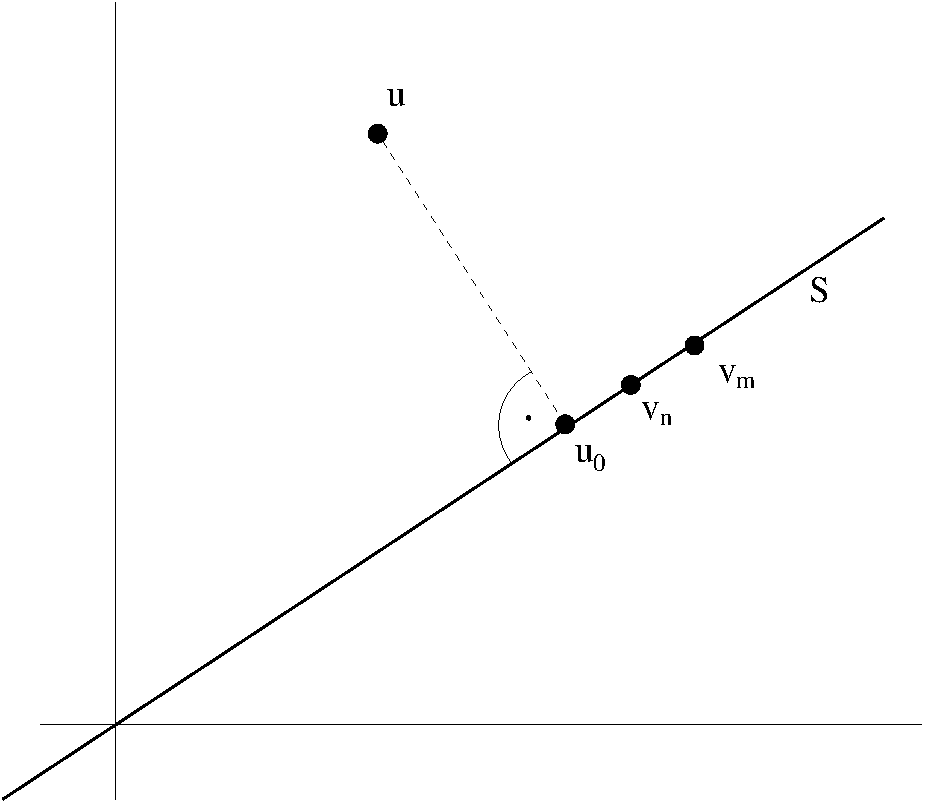
\includegraphics[height=4cm]{pictures/project}
\end{center}


We first check that there holds
$$
\| v_n - v_m \|^2 = 2 \, \| v_n - u \|^2 + 2 \, \| v_m - u \|^2 - 4 \,  \| \tfrac{1}{2}(v_n+v_m) - u \|^2.
$$
Since $1/2 (v_n+v_m) \in S$, there holds $\| 1/2 (v_n+v_m) - u \| \geq d$.
We proof that $(v_n)$ is a Cauchy sequence:
Fix $\eps > 0$, choose $N \in \setN$ such that for $n > N$ there holds
$\| u - v_n \|^2 \leq d^2 + \eps^2$. Thus for all $n,m > N$ there holds
$$
\| v_n - v_m \|^2 \leq 2 (d^2+\eps^2) + 2 (d^2 + \eps^2) - 4 d^2 = 4 \eps^2.
$$ 
Thus, $v_n$ converge to some $u_0 \in V$. Since $S$ is closed, $u_0 \in S$.
By continuity of the norm, $\| u - u_0 \| = d$.

\medskip
Fix some $0 \neq w \in S$, and define $\varphi(t) := \| u - \underbrace{u_0 - t w}_{\in S} \|^2$.
$\varphi(\cdot)$ is a convex function, it takes its unique minimum $d$ at $t=0$. Thus
$$
0 = \frac{d \varphi(t)}{dt}|_{t=0} = \{ 2 (u-u_0, w) - 2 t (w,w) \} |_{t=0} = 
   2 (u-u_0,w)
$$ 
We obtained $u-u_0 \bot S$. If there were two minimizers $u_0 \neq u_1$, 
then $u_0-u_1 = (u_0-u) - (u_1-u) \bot S$ and $u_0-u_1 \in S$, which implies
$u_0-u_1 = 0$, a contradiction.
\hfill $\Box$

\bigskip
Theorem~\ref{theo_proj} says that given an $u \in V$, we can uniquely
decompose it as
$$
u = u_0 + u_1, \qquad u_0 \in S \quad u_1 \in S^\bot
$$
This allows to define the operators $P_S : V \rightarrow S$ and $P_S^\bot : V \rightarrow S^\bot$ as 
$$
P_S u := u_0 \qquad P_S^\bot u := (I - P_S) u = u_1
$$

\begin{theorem} $P_S$ and $P_S^\bot$ are linear operators. 
\end{theorem}

\begin{definition} A linear operator $P$ is called a {\bf projection} if $P^2 = P$.
A projector is called {\bf orthogonal}, if $(Pu,v) = (u,Pv)$.
\end{definition}
\begin{lemma} The operators $P_S$ and $P_S^\bot$ are both orthogonal 
projectors.
\end{lemma}
\noindent
{\em Proof:} For $u \in S$ there holds $P_S u = u$. Since $P_S u \in S$, there holds $P_S^2 u = P_S u$. It is orthogonal since
$$
(P_Su,v) = (P_Su,v-P_Sv+P_Sv) = (\underbrace{P_S u}_{\in S}, \underbrace{v-P_Sv}_{\in S^\bot}) + (P_Su,P_Sv) = (P_Su,P_Sv).
$$
With the same argument there holds $(u,P_Sv) = (P_Su,P_Sv)$.
The co-projector $P_S^\bot = I - P_S$ is a projector since
$$
(I-P_S)^2 = I - 2 P_S + P_S^2 = I - P_S.
$$
It is orthogonal since $((I-P_S) u,v) = (u,v)-(P_Su,v) =
        (u,v)-(u,P_Sv) = (u,(I-P_S)v)$
\hfill $\Box$

\section{Riesz Representation Theorem}
Let $u \in V$. Then, we can define the related continuous linear
functional~$l_u(\cdot) \in V^\ast$ by
$$
l_u (v) := (u,v)_V \qquad \forall \, v \in V.
$$
The opposite is also true:
\begin{theorem} {\bf Riesz Representation Theorem.} Any continuous linear
functional $l$ on a Hilbert space $V$ can be represented uniquely as
\begin{equation}
\label{equ_rieszrep}
l(v) = (u_l,v)
\end{equation}
for some $u_l \in V$. Furthermore, we have
$$
\| l \|_{V^\ast} = \| u_l \|_V.
$$
\end{theorem}
\noindent
{\em Proof:} First, we show uniqueness. Assume that $u_1 \neq u_2$ both
fulfill (\ref{equ_rieszrep}). This leads to the contradiction
\begin{eqnarray*}
0 & = & l(u_1-u_2) - l(u_1-u_2) \\
  & = & (u_1,u_1-u2) - (u_2,u_1-u_2) = \| u_1 - u_2 \|^2.
\end{eqnarray*}
Next, we construct the $u_l$. For this, define 
$S := \operatorname{ker} l$. This is a closed subspace. 

\noindent
Case 1: $S^\bot = \{ 0 \}$. Then, $S = V$, i.e., $l = 0$. So take $u_l = 0$.

\noindent
Case 2: $S^\bot \neq \{ 0 \}$. Pick some $0 \neq z \in S^\bot$. There
holds $l(z) \neq 0$ (otherwise, $z \in S \cap S^\bot = \{ 0 \}$).
Now define 
$$
u_l := \frac{l(z)}{\|z\|^2} z \qquad \in S^\bot
$$
Then
\begin{eqnarray*}
(u_l,v) & = & (\underbrace{u_l}_{S^\bot}, \underbrace{v - l(v)/l(z) z}_S) + (u_l,l(v)/l(z)z) \\
& = & l(z) / \| z\|^2 (z,l(v)/l(z) z) \\
& = & l(v)
\end{eqnarray*}
Finally, we prove $\|l\|_{V^\ast} = \| u_l \|_V$:
$$
\|l\|_{V^\ast} = \sup_{0 \neq v \in V} \frac{l(v)}{\|v\|}
        = \sup_v \frac{(u_l,v)_V}{\|v\|_V} \leq \| u_l \|_V
$$
and
$$
\| u_l \| = \frac{l(z)}{\|z\|^2}  \|z\| = \frac{l(z)}{\|z\|} \leq \| l \|_{V^\ast}.
$$
% \hfill $\Box$

\section{Symmetric variational problems}
Take the function space $C^1(\Omega)$, and define the bilinear form
$$
A(u,v) := \int_\Omega \nabla u \nabla v + \int_\Gamma u v \, ds
$$
and the linear form
$$
f(v) := \int_\Omega f v \, dx
$$
The bilinear form is non-negative, and $A(u,u) = 0$ implies $u = 0$.
Thus $A(\cdot,\cdot)$ is an inner product, and provides the
norm $\|v\|_A := A(v,v)^{1/2}$. The normed vector space $(C^1, \|.\|_A)$
is not complete. Define
$$
V := \overline{C^1(\Omega)}^{\|.\|_A},
$$
which is a Hilbert space per definition. If we can show that there exists
a constant $c$ such that
$$
f(v) = \int_\Omega f v \, dx \leq c \| v \|_A \qquad \forall \, v \in V
$$
then $f(.)$ is a continuous linear functional on $V$.
We will prove this later. In this case, the Riesz representation theorem 
tells that there exists an unique $u \in V$ such that
$$
A(u,v) = f(v).
$$
This shows that the weak form has a unique solution in $V$.

Next, take the finite dimensional ($\Rightarrow$ closed) finite element subspace $V_h \subset V$.
The finite element solution $u_h \in V_h$ was defined by
$$
A(u_h,v_h) = f(v_h) \qquad \forall \, v_h \in V_h,
$$
This means
$$
A(u-u_h, v_h) = A(u,v_h) - A(u_h,v_h) = f(v_h) - f(v_h) = 0
$$
$u_h$ is the projection of $u$ onto $V_h$, i.e.,
$$
\| u - u_h \|_A \leq \| u - v_h \|_A \qquad \forall \, v_h \in V_h
$$
The error $u - u_h$ is orthogonal to $V_h$.

\section{Coercive variational problems}
%
In this chapter we discuss variational problems posed in Hilbert spaces.
Let $V$ be a Hilbert space, and let $A(\cdot,\cdot) : V \times V \rightarrow \setR$ be
a bilinear form which is
\begin{itemize}
\item coercive (also known as elliptic)
\begin{equation}
A(u,u) \geq \alpha_1 \| u \|_V^2 \qquad \forall \, u \in V,
\end{equation}
\item and continuous
\begin{equation}
A(u,v) \leq \alpha_2 \| u \|_V  \, \| v \|_V \qquad \forall \, u , v \in V,
\end{equation}
\end{itemize}
with bounds $\alpha_1$ and $\alpha_2$ in $\setR^+$. It is not necessarily symmetric.
Let $f(.) : V \rightarrow \setR$ be a continuous linear form on $V$, i.e., 
$$
f(v) \leq \| f \|_{V^\ast} \| v \|_V.
$$
We are posing the variational problem: find $u \in V$ such that
$$
A(u,v) = f(v) \qquad \forall \, v \in V.
$$

\begin{example} 
Diffusion-reaction equation: 
\end{example}
\noindent
Consider the PDE
$$
-\opdiv (a(x) \nabla u) + c(x) u = f \qquad \mbox{in } \Omega,
$$
with Neumann boundary conditions. Let $V$ be the Hilbert space generated 
by the inner product $(u,v)_V := (u,v)_{L_2}+ (\nabla u , \nabla v)_{L_2}$. 
The variational formulation of the PDE involves the bilinear form
$$
A(u,v) = \int_{\Omega} (a(x) \nabla u) \cdot \nabla v \, dx + \int_\Omega c(x) u v \, dx.
$$
Assume that the coefficients $a(x)$ and $c(x)$ fulfill 
$a(x) \in \setR^{d \times d}$, $a(x)$ symmetric and $\lambda_1 \leq \lambda_{\min} (a(x)) \leq \lambda_{\max} (a(x)) \leq \lambda_2$, and 
$c(x)$ such that $\gamma_1 \leq c(x) \leq \gamma_2$ almost everywhere. 
Then $A(\cdot,\cdot)$ is coercive with constant
$\alpha_1 = \min \{ \lambda_1, \gamma_1 \}$ and $\alpha_2 = \max \{ \lambda_2, \gamma_2 \}$.
\begin{example}  \label{example_diffconv}
Diffusion-convection-reaction equation:
\end{example}
\noindent
The partial differential equation
$$
-\Delta u + b \cdot \nabla u + u  = f \qquad \mbox{in} \; \Omega
$$
with Dirichlet boundary conditions $u = 0$ on $\partial \Omega$ leads to the
bilinear form
$$
A(u,v) = \int \nabla u \, \nabla v \, dx + \int b \cdot \nabla u \, v \, dx + \int u v \, dx.
$$
If $\opdiv b \leq 0$, what is an important case arising from incompressible flow
fields ($\opdiv \, b = 0$), then $A(\cdot,\cdot)$ is coercive and continuous w.r.t. the same norm as above.

\bigskip

Instead of the linear form $f(\cdot)$, we will often write $f \in V^\ast$. The evaluation is written as the duality product 
$$
\left< f , v \right>_{V^\ast \times V} = f(v).
$$

\begin{lemma}A continuous bilinear form $A(\cdot,\cdot) : V \times V \rightarrow \setR$
induces a continuous linear operator $A : V \rightarrow V^\ast$ via
$$
\left< A u, v \right> = A(u,v) \qquad \forall \, u,v \in V.
$$
The operator norm $\| A \|_{V \rightarrow V^\ast}$ is bounded by the continuity bound $\alpha_2$ of $A(\cdot,\cdot)$. 
\end{lemma}
\noindent
{\em Proof:} For every $u \in V$, $A(u,\cdot)$ is a bounded linear form on $V$
with norm
$$
\| A(u,\cdot) \|_{V^\ast} = 
\sup_{v \in V} \frac{A(u,v)}{ \| v \|_V} 
\leq \sup_{v \in V} \frac{\alpha_2 \| u \|_V \, \| v \|_V }{ \| v \|_V} 
= \alpha_2 \| u \|_V
$$
Thus, we can define the operator $A : u \in V \rightarrow A(u,\cdot) \in V^\ast$. 
It is linear, and its operator norm is bounded by
\begin{eqnarray*}
\| A \|_{V \rightarrow V^\ast} & = &
\sup_{u\in V} \frac{ \| A u \|_{V^\ast}}{\| u \|_V} =
\sup_{u\in V} \sup_{v \in V} \frac{ \left< A u, v\right>_{V^\ast \times V} } {\| u \|_V \, \| v \|_V} \\
& = & \sup_{u\in V} \sup_{v \in V} \frac{ A (u,v) } {\| u \|_V \, \| v \|_V} \leq
\sup_{u\in V} \sup_{v\in V} \frac{ \alpha_2 \| u \|_V \| v \|_V } {\| u \|_V \, \| v \|_V} = \alpha_2.
\end{eqnarray*}
\hfill $\Box$

Using this notation, we can write the variational problem as operator equation: find $u \in V$ such that
$$
A u = f \qquad (\mbox{in } V^\ast).
$$

\begin{theorem}[Banach's contraction mapping theorem] Given a Banach space
$V$ and a mapping $T : V \rightarrow V$, satisfying the Lipschitz condition
$$
\| T(v_1) - T(v_2) \| \leq L \, \| v_1 - v_2 \| \qquad \forall  \, v_1, v_2 \in V
$$
for a fixed $L \in [0,1)$. Then there exists a unique $u \in V$ such that
$$
u = T(u),
$$
i.e. the mapping $T$ has a unique fixed point $u$. The iteration $u^1 \in V$ given, compute
$$
u^{k+1} := T(u^k)
$$
converges to $u$ with convergence rate $L$:
$$
\| u - u^{k+1} \| \leq L \| u - u^k \|
$$
\end{theorem}


\begin{theorem}[Lax Milgram] Given a Hilbert space $V$, a coercive and continuous bilinear form $A(\cdot,\cdot)$, and a continuous linear form $f(.)$. Then there exists a unique $u \in V$ solving
$$
A(u,v) = f(v) \qquad \forall \, v \in V.
$$
There holds 
\begin{equation} \label{equ_lax_milgram_bound}
\| u \|_V \leq \alpha_1^{-1} \| f \|_{V^\ast}
\end{equation}
\end{theorem}
{\em Proof:} Start from the operator equation $A u = f$. Let $J_V : V^\ast \rightarrow V$ be the Riesz isomorphism defined by
$$
(J_V g, v)_V = g(v) \qquad \forall \, v \in V, \;  \forall \, g \in V^\ast.
$$
Then the operator equation is equivalent to
$$
J_V A u = J_V f \qquad (\mbox{in } V),
$$
and to the fixed point equation (with some $0 \neq \tau \in \setR$ chosen below)
\begin{equation} \label{equ_fixedpointequ}
u = u - \tau J_V (A u - f).
\end{equation}
We will verify that
$$
T (v) := v - \tau J_V (A v - f)
$$
is a contraction mapping, i.e., $\| T (v_1) - T (v_2) \|_V \leq L \| v_1 - v_2 \|_V$ 
with some Lipschitz constant $L \in [0,1)$.
Let $v_1, v_2 \in V$, and set $v = v_1 - v_2$. Then
\begin{eqnarray*}
\| T (v_1) - T (v_2) \|_V^2 
& = & \| \{ v_1 - \tau J_V (A v_1 - f) \} - \{ v_2 - \tau J_V (A v_2 -f) \} \|_V^2 \\
& = & \| v - \tau J_V A v \|_V^2 \\
& = & \| v \|_V^2 - 2 \tau (J_V A v, v)_V + \tau^2 \| J_V A v \|_V^2 \\
& = & \| v \|_V^2 - 2 \tau \left< A v , v \right> + \tau^2 \| A v \|_{V^\ast}^2 \\
& = & \| v \|_V^2 - 2 \tau A(v,v) + \tau^2 \| A v \|_{V^\ast}^2 \\
& \leq & \| v \|_V^2 - 2 \tau \alpha_1 \| v \|_V^2 + \tau^2 \alpha_2^2 \| v \|_V^2 \\
& = & (1 - 2 \tau \alpha_1 + \tau^2 \alpha_2^2) \| v_1 - v_2 \|_V^2
\end{eqnarray*}
Now, we choose $\tau = \alpha_1 / \alpha_2^2$, and obtain a Lipschitz constant
$$
L^2 = 1 - \alpha_1^2 / \alpha_2^2 \in [0,1).
$$
Banach's contraction mapping theorem state that (\ref{equ_fixedpointequ}) 
has a unique fixed point. Finally, we obtain the bound (\ref{equ_lax_milgram_bound}) from
$$
\| u \|_V^2 \leq \alpha_1^{-1} A(u,u) = \alpha_1^{-1} \, f(u) \leq \alpha_1^{-1} \| f\|_{V^\ast} \| u \|_V,
$$
and dividing by one factor $\|u\|$.
\hfill $\Box$

\subsection{Approximation of coercive variational problems}
Now, let $V_h$ be a closed subspace of $V$. We compute the
approximation $u_h \in V_h$ by the Galerkin method
\begin{equation}
A(u_h, v_h) = f(v_h) \qquad \forall \, v_h \in V_h.
\end{equation}
This variational problem is uniquely solvable by Lax-Milgram, 
since, $(V_h,\|.\|_V)$ is 
a Hilbert space, and continuity and coercivity on $V_h$ are inherited
from the original problem on $V$.


The next theorem says, that the solution defined by the Galerkin method is,
up to a constant factor, as good as the best possible approximation in the
finite dimensional space.

\begin{theorem}[Cea] The approximation error of the Galerkin method
is quasi optimal
$$
\| u - u_h \|_V \leq \alpha_2 / \alpha_1 \inf_{v \in V_h} \| u - v_h \|_V
$$
\end{theorem}
{\em Proof:} A fundamental property is the Galerkin orthogonality
$$
A(u-u_h, w_h) = A(u,w_h) - A(u_h, w_h) = f(w_h) - f(w_h) = 0
\qquad \forall \, w_h \in V_h.
$$
Now, pick an arbitrary $v_h \in V_h$, and bound
\begin{eqnarray*}
\| u - u_h \|_V^2 & \leq & \alpha_1^{-1} A(u-u_h, u-u_h) \\
& = & \alpha_1^{-1} A(u-u_h, u-v_h) + \alpha_1^{-1} A(u-u_h, \underbrace{v_h-u_h}_{\in V_h}) \\
& \leq &  \alpha_2 / \alpha_1 \, \| u - u_h \|_V \| u - v_h \|_V.
\end{eqnarray*}
Divide one factor $\|u - u_h\|$. Since $v_h \in V_h$ was arbitrary, the estimation
holds true also for the infimum in $V_h$.
\hfill $\Box$

\bigskip
If $A(\cdot,\cdot)$ is additionally symmetric, then it is an inner product. In this
case, the coercivity and continuity properties are equivalent to
$$
\alpha_1 \| u \|_V^2 \leq A(u,u) \leq \alpha_2 \, \| u \|_V^2
\qquad \forall \, u \in V.
$$
The generated norm $\|.\|_A$ is an equivalent norm to $\|.\|_V$. In the 
symmetric case, we can use the orthogonal projection with respect to 
$(.,.)_A$ to improve the bounds to
$$
\| u - u_h \|_V^2 \leq \alpha_1^{-1} \| u - u_h \|_A^2 \leq
        \alpha_1^{-1} \inf_{v_h \in V_h} \| u - v_h \|_A^2 \leq
        \alpha_2 / \alpha_1 \| u - v_h \|_V^2.
$$
The factor in the quasi-optimality estimate is now the square root of the
general, non-symmetric case.

\section{Inf-sup stable variational problems}

The coercivity condition is by no means a necessary condition for a
stable solvable system. A simple, stable problem with non-coercive
bilinear form is to choose $V = \setR^2$, and the bilinear form 
$B(u,v) = u_1 v_1 - u_2 v_2$. The solution of $B(u,v) = f^T v$ is 
$u_1 = f_1$ and $u_2 = -f_2$. We will follow the convention to call
coercive bilinear forms $A(\cdot,\cdot)$, and the more general ones $B(\cdot,\cdot)$.

Let $V$ and $W$ be Hilbert spaces, and $B(\cdot,\cdot) : V \times W \rightarrow \setR$ be a continuous bilinear form with bound
\begin{equation}
B(u,v) \leq \beta_2 \| u \|_V \| v \|_W \qquad \forall \, u \in V, \; \forall \, v \in W.
\end{equation}
The general condition is the {\bf inf-sup condition}
\begin{equation} \label{equ_infsup}
\inf_{u \in V \atop u \neq 0} \sup_{v \in W \atop v \neq 0}
\frac{ B(u,v) } { \| u \|_V \, \| v \|_W } \geq \beta_1.
\end{equation}

Define the linear operator $B : V \rightarrow W^\ast$ by $\left< B u, v \right>_{W^\ast \times W} = B(u,v)$. The inf-sup condition can be reformulated as
$$
\sup_{v \in W} \frac{ \left< B u, v \right> } { \| v \|_W } \geq \beta_1 \| u \|_V, \qquad \forall \, u \in V
$$
and, using the definition of the dual norm,
\begin{equation} \label{equ_stabb}
\| B u \|_{W^\ast} \geq \beta_1 \| u \|_V.
\end{equation}
We immediately obtain that $B$ is one to one, since
$$
B u = 0 \Rightarrow u = 0
$$
\begin{lemma} Assume that the continuous bilinear form $B(\cdot,\cdot)$ fulfills the
inf-sup condition (\ref{equ_infsup}). Then the according operator $B$ has
closed range.
\end{lemma}
{\em Proof:} Let $B u^n$ be a Cauchy sequence in $W^\ast$. From (\ref{equ_stabb}) we conclude that also $u^n$ is Cauchy in $V$. Since $V$ is complete, $u_n$
converges to some $u \in V$. By continuity of $B$, the sequence $B u^n$ converges to $B u \in W^\ast$.
\hfill $\Box$

The inf-sup condition (\ref{equ_infsup}) does not imply that $B$ is onto $W^\ast$. To insure that, we can pose an inf-sup condition the other way around:
\begin{equation} \label{equ_infsupb}
\inf_{v \in W \atop v \neq 0} \sup_{u \in V \atop u \neq 0}
\frac{ B(u,v) } { \| u \|_V \, \| v \|_W } \geq \beta_1.
\end{equation}
It will be sufficient to state the weaker condition
\begin{equation} \label{equ_infsup2}
\sup_{u \in V \atop u \neq 0}
\frac{ B(u,v) } { \| u \|_V \, \| v \|_W } > 0 \qquad \forall \, v \in W.
\end{equation}

\begin{theorem} \label{theo_infsup} 
Assume that the continuous bilinear form $B(\cdot,\cdot)$ fulfills
the inf-sup condition (\ref{equ_infsup}) and condition (\ref{equ_infsup2}). 
Then, the variational problem: find $u \in V$ such that
\begin{equation} \label{equ_bigsystem}
B(u,v) = f(v) \qquad \forall \, v \in W
\end{equation}
has a unique solution. The solution depends continuously on the right hand
side:
$$
\| u \|_V \leq \beta_1^{-1} \| f \|_{W^\ast}
$$
\end{theorem}
{\em Proof:} We have to show that the range $R(B) = W^\ast$. The Hilbert
space $W^\ast$ can be split into the orthogonal, closed subspaces
$$
W^\ast = R(B) \oplus R(B)^\bot.
$$
Assume that there exists some $0 \neq g \in R(B)^\bot$. This means that
$$
(B u, g)_{W^\ast} = 0 \qquad \forall \, u \in V.
$$
Let $v_g \in W$ be the Riesz representation of $g$, i.e., $(v_g, w)_W = g(w)$ for all $w \in W$. This $v_g$ is in contradiction to the assumption 
(\ref{equ_infsup2})
$$
\sup_{u \in V} \frac{B(u,v_g)}{ \| u \|_V} = 
\sup_{u \in V} \frac{(Bu,g)_{W^\ast}}{ \| u \|_V} = 
0.
$$
Thus, $R(B)^\bot = \{ 0 \}$ and $R(B) = W^\ast$.
\hfill $\Box$

\begin{example}A coercive bilinear form is inf-sup stable.
\end{example}
\begin{example}A complex symmetric variational problem:
\end{example}
\noindent
Consider the complex valued PDE 
$$
-\Delta u + i u = f,
$$
with Dirichlet boundary conditions, $f \in L_2$, and $i = \sqrt{-1}$. The
weak form for the real system $u = (u_{r}, u_i) \in V^2$ is
\begin{equation}
\begin{array}{rcll}
(\nabla u_{r}, \nabla v_{r})_{L_2} + (u_i, v_{r})_{L_2} & = &
        (f,v_{r}) \qquad & \forall \, v_r \in V \\
(u_{r}, v_i)_{L_2} -(\nabla u_i, \nabla v_i)_{L_2} & = &
        -(f,v_i) & \forall \, v_i \in V
\end{array}
\end{equation}
We can add up both lines, and define the large bilinear form $B(\cdot,\cdot) : V^2 \times V^2 \rightarrow \setR$ by
$$
B ((u_r,u_i), (v_r, v_i)) = 
(\nabla u_{r}, \nabla v_{r}) + (u_i, v_{r}) + (u_{r}, v_i) -(\nabla u_i, \nabla v_i)
$$
With respect to the norm $\|v\|_V = ( \| v \|_{L_2}^2 + \| \nabla v \|_{L_2}^2)^{1/2}$, the bilinear form is continuous, and fulfills the inf-sup conditions
(exercises !)
Thus, the variational formulation: find $u \in V^2$ such that
$$
B(u,v) = (f,v_r) - (f,v_i) \qquad \forall \, v \in V^2
$$
is stable solvable.

\bigskip

\subsection{Approximation of inf-sup stable variational problems}
Again, to approximate (\ref{equ_bigsystem}), we pick finite dimensional
subspaces $V_h \subset V$ and $W_h \subset W$, and pose the finite dimensional
variational problem: find $u_h \in V_h$ such that
$$
B(u_h, v_h) = f(v_h) \qquad \forall \, v_h \in W_h.
$$
But now, in contrast to the coercive case, the solvability of the 
finite dimensional equation does not follow from the solvability conditions
of the original problem on $V \times W$. E.g., take the example in $\setR^2$
above, and choose the subspaces $V_h = W_h = \mbox{span} \{ (1,1) \}$. 

We have to pose an extra inf-sup condition for the discrete problem:
\begin{equation} \label{equ_infsuph}
\inf_{u_h \in V_h \atop u_h \neq 0} \sup_{v_h \in W_h \atop v_h \neq 0}
\frac{ B(u_h,v_h) } { \| u_h \|_V \, \| v_h \|_W } \geq \beta_{1h}.
\end{equation}
On a finite dimensional space, one to one is equivalent to onto, and we
can skip the second condition.

\begin{theorem} \label{theo_approxinfsup}
Assume that $B(\cdot,\cdot)$ is continuous with bound $\beta_2$, and 
$B(\cdot,\cdot)$ fulfills the discrete inf-sup condition with bound $\beta_{1h}$. 
Then there holds the quasi-optimal error estimate
\begin{equation}
\| u - u_h \| \leq (1 + \beta_2 / \beta_{1h}) \inf_{v_h \in V_h} \| u - v_h \|
\end{equation}
\end{theorem}
\noindent
{\em Proof:} Again, there holds the Galerkin orthogonality $B(u,w_h) = B(u_h,w_h)$ for all $w_h \in V_h$. Again, choose an arbitrary $v_h \in V_h$:
\begin{eqnarray*}
\| u - u_h \|_V & \leq & \| u - v_h \|_V + \| v_h - u_h \|_V \\
        & \leq & \| u - v_h \|_V + \beta_{1h}^{-1} 
                \sup_{w_h \in W_h} \frac{ B(v_h-u_h, w_h) } { \| w_h \|_V } \\
        & = &  \| u - v_h \|_V + \beta_{1h}^{-1} 
                \sup_{w_h \in W_h} \frac{ B(v_h-u, w_h) } { \| w_h \|_V } \\
        & \leq & \| u - v_h \|_V + \beta_{1h}^{-1}
                \sup_{w_h \in W_h} \frac{ \beta_2 \| v_h-u \|_V \, \| w_h \|_W } { \| w_h \|_W } \\
        & = & (1 + \beta_2 / \beta_{1h}) \| u - v_h\|_V.
\end{eqnarray*}
